\documentclass[a4paper,10pt]{article}
\usepackage[british]{babel}
\usepackage[T1]{fontenc}
\usepackage[hidelinks]{hyperref}
\usepackage[a4paper]{geometry}

\usepackage{tabularx}
\usepackage{graphicx}
\usepackage{rotating}
\usepackage{float}
\usepackage{xspace}

% Math packages
\usepackage[sc]{mathpazo}
\usepackage{amsthm}
\usepackage{algorithmic}
\usepackage{amsmath}

\usepackage{listings}

% Document properties
\title{Welch-Lynch clock synchronization protocol \\\textit{Modelling in UPPAAL}}
\author{
	Wouter Geraedts \\ \small{\texttt{w.geraedts@student.ru.nl}} \and
	Ko Stoffelen     \\ \small{\texttt{kostoffelen@student.ru.nl}}
}
\date{}
\linespread{1.05}

% Terminology
\newcommand{\UPPAAL}{UPPAAL\xspace}

\begin{document}
	\maketitle

%%% Contents %%%
%Originele paper

%Zoeken naar concrete constanten

%Aanpassingen voor snelheid
%	Gebruik van C-functies [step1]
%	Gebruik van select-statements [step2]
%	Gebruik van local_time uit originele paper [step3]
%	Gebruik van SUM uit originele paper [step3minimized]
%	Timejumps [step3minimized]
%	Scalarset reduction [step4scalar]
%	Uitgebreide guards (forall i.p.v. local var C) [step2]

%Aanpassingen voor generiekerheid
%	Diff variable upgrade
%	Min en max (zelfs trager dan SUM) [step4]

%Resultaten: Vergelijkingen in performance
%Faulty process, niet mogelijk
%	Werk om te doen om het alsnog te maken (array voor min en max; zorgen dat het kan met scalarset (id_t))

\section{Introduction}

%Over dit paper
%Relatie met originele paper
%Opbouw van dit paper
%Korte verwijzing naar conclusie

This report is part of an assignment for the Analysis of Embedded Systems course in 2012--2013. Our goal was to model and analyze the Welch-Lynch fault-tolerant clock synchronization protocol \cite{Welch1984Anew} using \UPPAAL. A previous attempt has been made in 2004 \cite{Aceto2004Notes}, when the model had to be greatly simplified. New \UPPAAL features like symmetry reduction, a richer syntax and a more powerful verification engine in general, make that the model-based analysis deserved another chance.

The algorithm in its most general form still does not directly translate to an \UPPAAL model that is actually verifiable. This report first describes what optimizations, simplifications and updates have been applied to a general model. Then in section~\ref{sec:faulty} it is explained what else would have been needed to be able to verify a general version of the protocol. In section~\ref{sec:remarks} some remarks are made on \cite{Aceto2004Notes}, which explain some troubles that appeared in the process of this analysis. Next, our models are examined alongside the quality criteria for \UPPAAL models. Finally in section~\ref{sec:performance}, the performance of our optimized model is compared to the 2004 version, after which we draw our conclusions. \UPPAAL is able to verify the correctness of the protocol for three participating processes with a highly optimized model, but then we are already approaching the limit of \UPPAAL{}s capabilities.

\section{Optimizations}

In 2004, a model was made that models the protocol in almost its most general form. However, fault-tolerance is completely ignored and a trick is applied to model the floating point numbers that correspond to clocks. This has been our starting point of reference. The most important automaton, the description of a process, can be seen in figure~\ref{fig:original_process}.

\begin{figure}[!h]
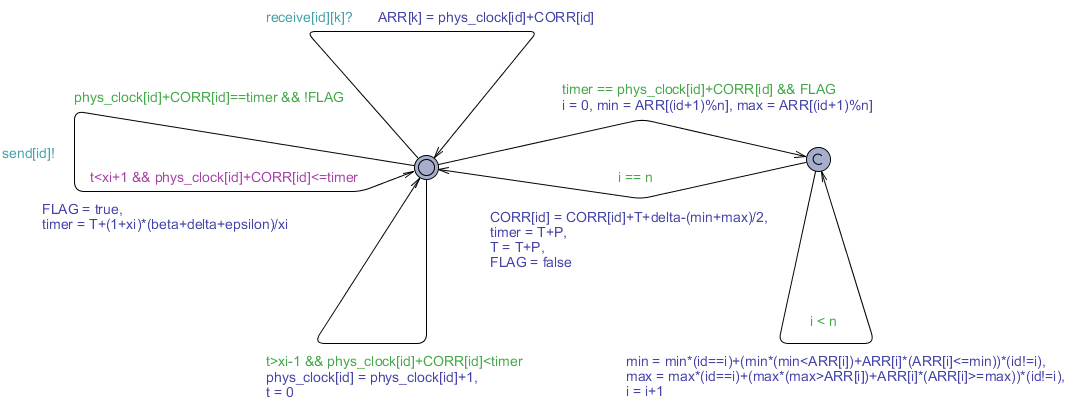
\includegraphics[width=\textwidth]{original_process}
\caption{Process in \texttt{original.xml}\label{fig:original_process}}
\end{figure}

It was soon getting clear that all other optimizations had to be applied as well and even additional ones. Below is a complete list of all optimization steps that have been used and how they contribute to making the model verifiable.

\begin{enumerate}
\item \textbf{C-like functions} \\
	The \UPPAAL C-like declaration language has been enriched extensively over the years. For instance, in 2004, one was not able to use functions and complicated constructions had to be thought off to simulate the behavior. In figure~\ref{fig:original_process}, the right part uses a committed state to iterate over an array to determine its minimal and maximal values. A similar structure is seen in the channel automaton. Luckily the new syntax allows us to replace these structures by C-like functions. Due to the nature of a committed state, this does not directly highly decrease the state space, but it allows for the removal of some variables, transitions and complex update statements. This makes the model more comprehensible. The removal of the variables \texttt{min} and \texttt{max} then does result in a decreased state space. The result can be seen in figure~\ref{fig:step1_process}.

\begin{figure}[!h]
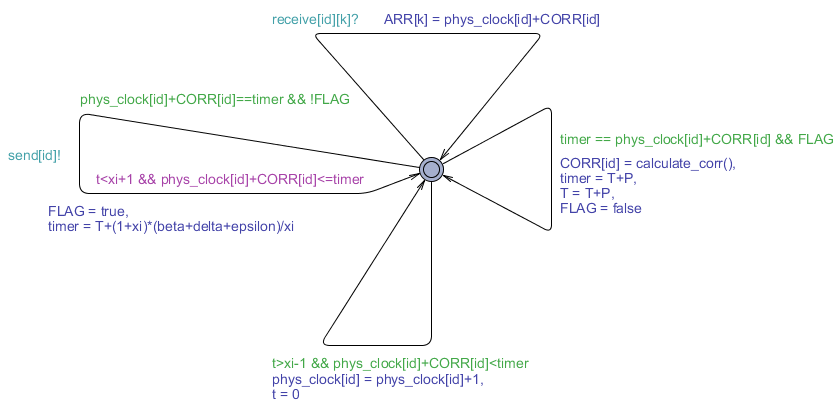
\includegraphics[width=\textwidth]{step1_process}
\caption{Process in \texttt{step1.xml}\label{fig:step1_process}}
\end{figure}

\item \textbf{Select statements} \\
	The 2004 model uses two \textit{choice variable} automatons to let each process and each channel non-deterministically choose which message to receive. The automatons are used to iterate over all process instances. Such choice variables can now easily be replaced by select statements that range over some type \texttt{id\_t}. This reduces the state space. All iterating is now done implicitly within one single transition, without branching the search space.

\item \textbf{Rewriting variables} \\
	The \UPPAAL verification engine can not deal with unbounded integers very well. To solve this, it was proposed in 2004 to rewrite lots of variables in such a way that one can work with bounded variables. The main idea is to introduce the notion of a round explicitly in the description of a process. This is implemented by subtracting the round index multiplied with the time between rounds from all timer variables. Now effectively, these timers can only take values up to the time between rounds, a constant \(P\). Then some invariants are used to further reduce the number of variables. The correctness property is also altered by this, but it can be proven that the systems are equivalent.

\item \textbf{Specific three process instance} \\
	In 2004, it was presumably noticed that it turned out to be hard to verify instances of the protocol using \UPPAAL. Therefore, the researchers tried to restrict themselves to three processes. This allows for a more direct computation of the minimum and maximum values in the right part of the process automaton. The variables \texttt{ARR1}, \texttt{min1} and \texttt{max1} are replaced by a single variable \texttt{SUM}. Removing variables implies reducing the search space.

\item \textbf{Time jumps} \\
	When traces were simulated within the model, it was noticed that for the larger part of the time, most variables were not changing values, except for the \texttt{local\_time} variable which was simply incrementing. When the counter reached 0, all process instances started to send out and receive messages. Before and after that, nothing changed within the system. This lead to the invention of a time jump optimization, where a process is allowed to simply skip the parts where nothing interesting is happening. Of course it has been made sure that the time jumps do not influence the total behavior of the system in any way. This optimization has been shown to greatly reduce the state space. The resulting process automaton can be seen in figure~\ref{fig:step3minimized_process}.

\begin{figure}[!h]
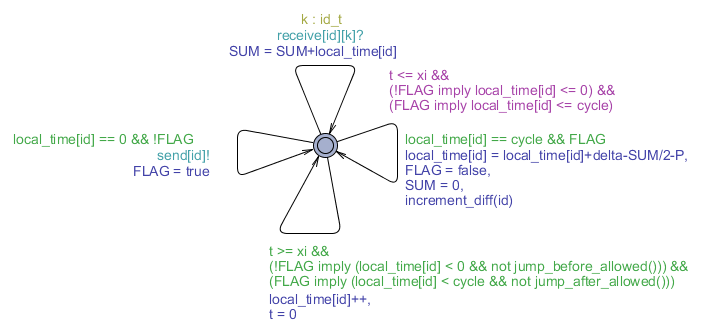
\includegraphics[width=\textwidth]{step3minimized_process}
\caption{Process in \texttt{step3minimized.xml}\label{fig:step3minimized_process}}
\end{figure}

\item \textbf{Symmetry reduction} \\
	Symmetry reduction \cite{Hendriks2004Adding} is a powerful technique to drastically reduce both computation time and memory usage. This reduction is exponential in the size of the scalar sets, a symmetric data type, that are used. The processes in the protocol are highly symmetrical. When their IDs are defined as a scalar set type, the \UPPAAL verifier can use so-called \textit{state swaps} to reduce the state space. For instance, there are different orders in which the \texttt{local\_time} counter can be incremented. Using symmetry reduction, the branching resulting from this ordering is reduced.

\item \textbf{Extended guards} \\
	The channel automaton used to contain a variable \(C\) that counted how many messages had been received. When all messages had been received, another transition could be taken. This variable has been removed completely, due to a richer syntax which allows for guards with \texttt{forall} modifiers. Now it's easier to check if all messages have been received, i.e. if all boolean values in an array are set to true. In figure~\ref{fig:original_channel}, one can see the original channel, while figure~\ref{fig:step4scalar_channel} shows the optimized automaton.

\begin{figure}[!h]
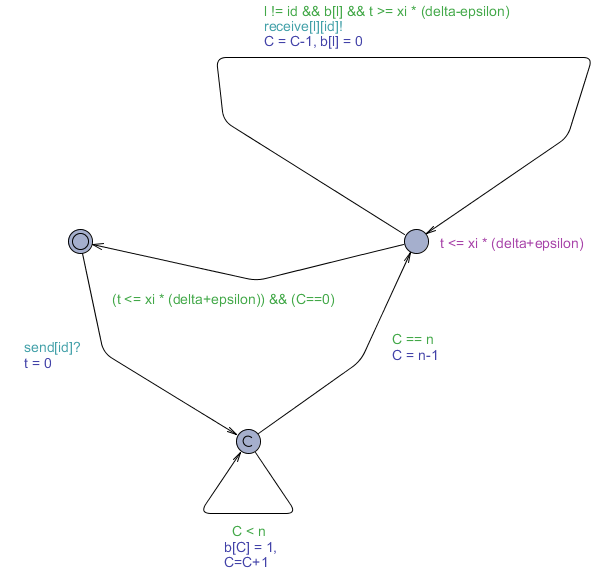
\includegraphics[scale=0.7]{original_channel}
\caption{Channel in \texttt{original.xml}\label{fig:original_channel}}
\end{figure}

\begin{figure}[!h]
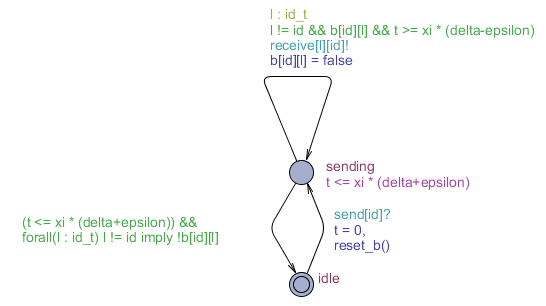
\includegraphics{step4scalar_channel}
\caption{Channel in \texttt{step4scalar.xml}\label{fig:step4scalar_channel}}
\end{figure}

\end{enumerate}

%Aanpassingen voor snelheid

\section{Towards faulty process\label{sec:faulty}}

Our highly optimized model turned out to be verifiable, as turns out in section~\ref{sec:performance}. However, this is only under the assumption of no faulty processes. It would certainly be interesting to put the fault-tolerance to the test. In \cite{Welch1984Anew} it is claimed that the protocol works correctly when there are at least \(3f+1\) processes in the system, where \(f\) is the number of faulty processes. The first interesting case, \(f=1\), still means that there have to be at least four processes, which we won't be able to calculate. The only thing we could do was to make our models easier extendible. We applied two changes to manage this.

%Aanpassingen voor generiekerheid

\begin{enumerate}
\item \textbf{\texttt{diff} variable} \\
	The optimized 2004 model contains a \texttt{diff} variable with an update statement that appears complicated. This statement computes the round difference between two specific processes, which is either -1, 0 or 1. This variable is used to verify models using the \texttt{local\_time} optimization, and can only be used for checking the processes with ids 0 and 1. In order to generalize this for all processes, and for the usage of scalarsets in which we can not explicitly refer to processes 0 and 1, a C-like function was introduced to compute the relative round differences compared to the process in the highest round, i.e. with the highest \texttt{diff} value. This update results in a bigger state space, as a diff-value for each process is introduced; instead of a single diff-value for the entire model. This penalty can be somewhat mitigated by the now possible use of scalarsets.

\item \textbf{Removing \texttt{SUM}} \\
	The introduction of a single \texttt{SUM} variable in our optimization list might be more efficient, but it's not usable when four or more processes are used. This is why we removed it and record a minimal and maximal value during the receiving of messages. This increases the state space by one variable, and paves the way for more then three processes.
\end{enumerate}

If we would have been able to calculate a system with four processes, we would have implemented the following two steps:

%Aanpassingen die we nog wilde doen, indien we 4 processen hadden kunnen modelleren

\begin{enumerate}
\item \textbf{Upgrading \texttt{MIN} and \texttt{MAX} to arrays} \\
	We would have upgraded the \texttt{MIN} and \texttt{MAX} variables to arrays with a length of $f+1$. In the case of $f=1$, we would have stored the top and bottom two timings per process, and averaged the lowest \texttt{MAX} en highest \texttt{MIN} values. This would result in actually ignoring the outliers, thus encompassing the fault-tolerant property of this protocol.
	
	Because we were never able to verify the model with four processes, we could never even begin to verify the protocol in the case of a single process ($f=1$). Thus the arrays with length $1$ are sufficient.
	
\item \textbf{Faulty process} \\
	And finally, we would have added a faulty process to the system, which is able to send or claim to have received messages at any time. In the case of scalarsets, because not a single process can be singled out, all processes would have to be able to become faulty. But, at most $f$ processes at any given time would be faulty.
	
	Because all outliers are filtered out, this should have no impact on the protocol. Because we can verify at most three processes, we can not model any faulty processes, because with $n = 3, n = 3f+1 \Rightarrow f=0$.
	
\end{enumerate}

\section{Remarks on \cite{Aceto2004Notes}\label{sec:remarks}}

In the process of our analysis, we have been troubled by some ambiguities that arose from \cite{Aceto2004Notes}. Again, these are enumerated below.

\begin{enumerate}
\item \textbf{Unclear what is computable} \\
	The paper does not claim what has actually been computable. It does not claim to have successfully verified any property. This made it hard for us to know what to expect. We hoped to go a bit further than only three processes. In the end, it appears that Aceto et al. \cite{Aceto2004Notes} were not able to verify the system for three processes; as we were not able to verify our copy of their model at all.

\item \textbf{No constant values} \\
	The protocol depends on a number of constants: \(\xi\), \(\delta\), \(\epsilon\), \(P\) and \(\beta\). Some constraints have been derived on these constants for the algorithm to work correctly:
	\[ (2(\beta+\epsilon)+\textrm{max}(\delta,\beta+\epsilon))\frac{\xi+1}{\xi} + \frac{\delta}{\epsilon} < P \le (\frac{\beta}{4}-\epsilon)\xi + \frac{\beta+\delta+\epsilon}{\xi}-2\beta-\delta-2\epsilon \]
	As no specific values that fulfil these constraints are given anywhere, it actually turned out to be non-trivial what values to pick. We first tried to verify this constraint in \UPPAAL itself, but it then turned out that \UPPAAL{}s integer division affected the upper bound in such a way that the property could not get satisfied. We were looking for a set of values that were as small as possible and we finally settled on a seemingly arbitrary \(\xi=80\), \(\delta=2\), \(\epsilon=1\), \(P=22\) and \(\beta=6\). We assumed that the constraints are derived correctly and we computed that this set of values satisfy the constraints.

\item \textbf{Variable types} \\
	In the paper, only pictures of models can be seen, not all declarations that are made in \UPPAAL. This made it in some instances unclear what the types of certain variables should have been. It also caused minor problems for making the types bounded. We ended up with a \texttt{typedef int[\(-P+\text{cycle}/2+\delta\), cycle] cycle\_t}, where \texttt{cycle} = \(\frac{\xi+1}{\xi}(\beta+\delta+\epsilon)\), by deriving the bounds ourselves, but it would definitely have been easier if this information had been available anywhere.
\end{enumerate}

%Niet duidelijk of ze daadwerkelijk het model hebben kunnen doorrekenen
%Geen concrete waarden voor constanten; beschrijving van zoektocht
%Onduidelijk wat het type is van variablen

\section{Quality\label{sec:quality}}

%Toelichten dat het leesbaarder is a.d.v. A First Introduction to UPPAAL

We compare our models to the guidelines stated at the end of ''A First Introduction to UPPAAL``. \cite{Vaandrager2011First}

\begin{enumerate}
\item \textbf{Object of modelling} \\
	In our most complex model, \texttt{step4scalar}, we have three distinct automata: a Process, which models a physical process in a network; a Channel, which models the physical characteristics of a broadcast channel in a network; and finally, the Helper, which models the virtual act of jumping through time.
\item \textbf{Purpose} \\
	We have built upon models which are descriptive, and serve to eventually verify the Welch-Lynch clock synchronization protocol. Specifically, we wish to verify the faulty-tolerance property of the protocol.
\item \textbf{Traceable} \\
	As explained before; the Process and Channel correspond to the physical aspects of the protocol; whereas the Helper corresponds to the virtual act of jumping through time, and thus encodes the explicit assumption that jumping through time in this manner does not change the behavior of the protocol. For links to the definition of the protocol we refer to the notes by Aceto et al. \cite{Aceto2004Notes}
\item \textbf{Truthful} \\
	Our model is not truthful in the sense that it explicitly encompasses behavior not possible in the real object of modelling: jumping through time. However, we have made this an explicit assumption, and thus should be considered acceptable. Our model is completely based on the notes of Aceto et al., and is thus at most as truthful as their model.
\item \textbf{Simple} \\
	We have simplified the original model considerably by using new \UPPAAL features such as \texttt{select}-statements, advanced guards and C-functions. Because of this a lot of administrative work done in the automata is now done by \UPPAAL or C-functions. This makes the models more readable, and conveniently reduces the state space in some cases.
\item \textbf{Extensible and reusable} \\
	In our last version of our model, \texttt{step4scalar}, we can arbitrarily increase the total number of processes in the model by increasing a single constant value. Also, the timing constraints can be adjusted by editing the appropriate constants. Lastly, because our model is simple, new components can be added easily. (For an example, see the Helper-automata)
\item \textbf{Interoperability and sharing} \\
	As we optimized our models pretty thoroughly, and has thus become a high abstraction of the original protocol, we doubt the model can be used for anything else other than verification. As such, our models are not very shareable.
\end{enumerate}

\section{Performance\label{sec:performance}}

%	Gebruik van C-functies [step1]
%	Gebruik van select-statements [step2]
%	Gebruik van local_time uit originele paper [step3]
%	Gebruik van SUM uit originele paper [step3minimized]
%	Timejumps [step3minimized]
%	Scalarset reduction [step4scalar]
%	Uitgebreide guards (forall i.p.v. local var C) [step2]

Over time we have implemented various improvements over the original model by Aceto et al. These improvements are:

\begin{enumerate}
\item various C-functions instead of for-loops in automata
\item select-statements instead of Choice automata
\item \texttt{local\_time} as improvement over \texttt{phys\_clock}
\item \texttt{sum} as improvement over \texttt{ARR}
\item time jumps to skip uninteresting time
\item \texttt{min} and \texttt{max} as more general alternative to \texttt{sum}; note that this improvement relatively increases the state space
\item scalarset reduction
\end{enumerate}

To measure the relative performance of each model, we ran the models on a machine with 4 GiB ram, and no swap memory. If using \UPPAAL and breadth first search the machine ran out of memory, we declared the model practically \emph{uncomputable}.

\vspace{1 em}

\begin{tabular}{|l|c|l|l|}
\hline
\textbf{model} & \textbf{$N$} & \textbf{time} & \textbf{improvements} \\ \hline
original & 3 & uncomputable & \\ \hline
originalfinal & 3 & uncomputable & 3, 4 \\ \hline
step1 & 3 & uncomputable & 1 \\ \hline
step2 & 3 & uncomputable & 1, 2 \\ \hline
step3 & 3 & uncomputable & 1, 2, 3 \\ \hline
step3scalar & 3 & uncomputable & 1, 2, 3, 7 \\ \hline
step3minimized & 3 & 105 seconds & 1, 2, 3, 4, 5 \\ \hline
step3scalarminimized & 3 & 35 seconds & 1, 2, 3, 4, 5, 7 \\ \hline
step4 & 3 & 220 seconds & 1, 2, 3, 5, 6\\ \hline
step4scalar & 3 & 40 seconds & 1, 2, 3, 5, 6, 7 \\ \hline
step4scalar & 4 & uncomputable & 1, 2, 3, 5, 6, 7 \\ \hline
\end{tabular}

%Vergelijking tussen verschillende versies van ons, en uiteindelijke versie van aceto2004notes

\section{Conclusion}
	
%We kunnen succesvol 3 processen door laten rekenen, sneller dan toen (40 sec vs. NIET)
%Als 4 haalbaar blijkt te zijn, dan dat.
%5 nodig voor Faulty Process-eigenschap.

From the above results above, we can conclude that the 'time jump'-improvement and replacement of \texttt{ARR} results in a practically computable model for the Welch-Lynch clock synchronization protocol for three processes. Regretfully we are still not able to verify the algorithm for more than three processes; let alone a faulty process.

Still, compared to the experiments of Aceto et al., our improvements on the model, more computational power, and the improvements on UPPAAL have made the verification of this protocol practical.

\bibliographystyle{plain}
\bibliography{main}

\end{document}
